\documentclass[11pt,a4paper]{article}
\usepackage[utf8]{inputenc}
\usepackage[english]{babel}
\usepackage{graphicx}
\usepackage{hyperref}
\usepackage{listings}
\usepackage{xcolor}
\usepackage{geometry}
\usepackage{amsmath}
\usepackage{float}
\usepackage{caption}
\usepackage{textcomp}
\usepackage[T1]{fontenc}
\usepackage{booktabs}
\usepackage{multirow}
\usepackage{tikz}
\usetikzlibrary{shapes.geometric, arrows.meta, positioning, fit, backgrounds}

\geometry{margin=1in}

\definecolor{codegreen}{rgb}{0,0.6,0}
\definecolor{codegray}{rgb}{0.5,0.5,0.5}
\definecolor{codepurple}{rgb}{0.58,0,0.82}
\definecolor{backcolour}{rgb}{0.95,0.95,0.92}
\definecolor{infrablue}{rgb}{0.88,0.95,1.0}
\definecolor{coreorange}{rgb}{1.0,0.95,0.88}
\definecolor{agentpurple}{rgb}{0.95,0.90,0.96}
\definecolor{toolgreen}{rgb}{0.91,0.96,0.91}
\definecolor{knowledgepink}{rgb}{0.99,0.89,0.93}

\lstdefinestyle{mystyle}{
    backgroundcolor=\color{backcolour},
    commentstyle=\color{codegreen},
    keywordstyle=\color{magenta},
    numberstyle=\tiny\color{codegray},
    stringstyle=\color{codepurple},
    basicstyle=\ttfamily\footnotesize,
    breakatwhitespace=false,
    breaklines=true,
    captionpos=b,
    keepspaces=true,
    numbers=left,
    numbersep=5pt,
    showspaces=false,
    showstringspaces=false,
    showtabs=false,
    tabsize=2,
    escapechar=@
}

\lstset{style=mystyle}

\title{\textbf{NATO Smart City IoT -- Q1 2026 Progress Report}\\
\large University of Mons}
\author{Tanguy Vansnick, Mathis Delehouzée, Islam Hentous, Saïd Mahmoudi}
\date{\today}

\begin{document}

\maketitle
\begin{abstract}
This report documents the Q1 2026 developments on the NATO IoT Attack Path Analysis platform. The system has been redesigned around a YAML-driven infrastructure model, a NetworkX directed graph backend, and a multi-phase LLM agent pipeline that automates the full pentest workflow: topology analysis, network reconnaissance, vulnerability analysis, exploitation validation, and report generation. New additions include Dijkstra-based weighted attack path analysis, a ChromaDB-backed knowledge store with semantic search, declarative hardware attack tool definitions (HackRF One, Flipper Zero, Proxmark3, Exploit IoT Kit), and a multi-provider LLM abstraction supporting Anthropic, OpenRouter, and other providers. The pipeline has been validated on the physical lab, producing actionable findings including anonymous MQTT access, legacy SSH/nginx vulnerabilities, and multi-hop attack chains.
\end{abstract}

% ================================================================
\section{Changes from Q4 2025}
% ================================================================

The platform has undergone a complete architectural redesign since Q4 2025. The previous system relied on a Neo4j graph database with MongoDB caching and MCP/Ollama integration for AI queries. Q1 2026 replaces this with a streamlined, in-process architecture centered on a multi-phase LLM agent pipeline. Table~\ref{tab:changes} summarizes the key changes.

\begin{table}[H]
\centering
\begin{tabular}{@{}lll@{}}
\toprule
\textbf{Component} & \textbf{Q4 2025} & \textbf{Q1 2026} \\
\midrule
Infrastructure format & JSON & YAML (single source of truth) \\
Graph database & Neo4j (external) & NetworkX DiGraph (in-process) \\
Cache layer & MongoDB & ChromaDB (vector DB with embeddings) \\
CVE enrichment & Custom NVD client & NVD client + CPE mapping YAML \\
AI integration & MCP Neo4j + Ollama & Multi-phase LLM agent pipeline \\
Attack paths & Basic graph traversal & Dijkstra-weighted (CVSS + protocol) \\
Tool definitions & Hardcoded Python & Declarative YAML (software + hardware) \\
Risk scoring & CVSS only & CVSS + hop distance + betweenness centrality \\
Lab environment & Simulated JSON topology & Real physical lab (192.xxx.x.0/24) \\
Testing & Manual validation & 193 automated tests (14 files) \\
\bottomrule
\end{tabular}
\caption{Architecture evolution from Q4 2025 to Q1 2026}
\label{tab:changes}
\end{table}

Each change was driven by a specific rationale:

\begin{itemize}
    \item \textbf{Neo4j $\rightarrow$ NetworkX}: The lab topology (15 devices, 16 links) does not justify an external database server. NetworkX provides equivalent query capabilities in-process (BFS, Dijkstra, centrality) without operational overhead. The abstract \texttt{GraphBackend} ABC preserves the ability to swap in Neo4j or Memgraph for larger deployments.
    \item \textbf{MongoDB $\rightarrow$ ChromaDB}: Moving from key-value caching to a vector database enables \emph{semantic search} over security knowledge. Agents can query ``zigbee RF sniffing attack'' and retrieve relevant methodology chunks, rather than requiring exact key matches.
    \item \textbf{JSON $\rightarrow$ YAML}: YAML is more readable for infrastructure definitions and supports comments for documentation. A single YAML file serves as the source of truth, consumed by the graph builder, visualization, and agent pipeline.
    \item \textbf{MCP/Ollama $\rightarrow$ Agent pipeline}: The Q4 single-query MCP approach could not perform multi-step reasoning (scan, then analyze, then correlate). The 5-phase pipeline decomposes the pentest into specialized agents that pass deliverables between phases, enabling compound analysis.
    \item \textbf{Hardcoded tools $\rightarrow$ Declarative YAML}: Adding a new recon tool (e.g., \texttt{nikto}) requires only a YAML file --- no Python code changes. Hardware tools use the same format with a \texttt{type: hardware} marker.
    \item \textbf{Simulated $\rightarrow$ Real lab}: Active reconnaissance on physical devices (nmap, ssh-audit, mqtt\_listen) reveals discrepancies between documented and actual configurations, producing higher-fidelity findings.
\end{itemize}

% ================================================================
\section{Physical Lab Infrastructure}
% ================================================================

Unlike Q4 2025, which operated on simulated JSON topologies, the Q1 2026 platform models a \textbf{real physical IoT lab} on subnet 192.xxx.x.0/24. The lab contains 15 devices interconnected through Ethernet, LoRaWAN (EU868), Zigbee (802.15.4), MQTT, and WAN links.

\subsection{Network Topology}

\begin{figure}[H]
\centering
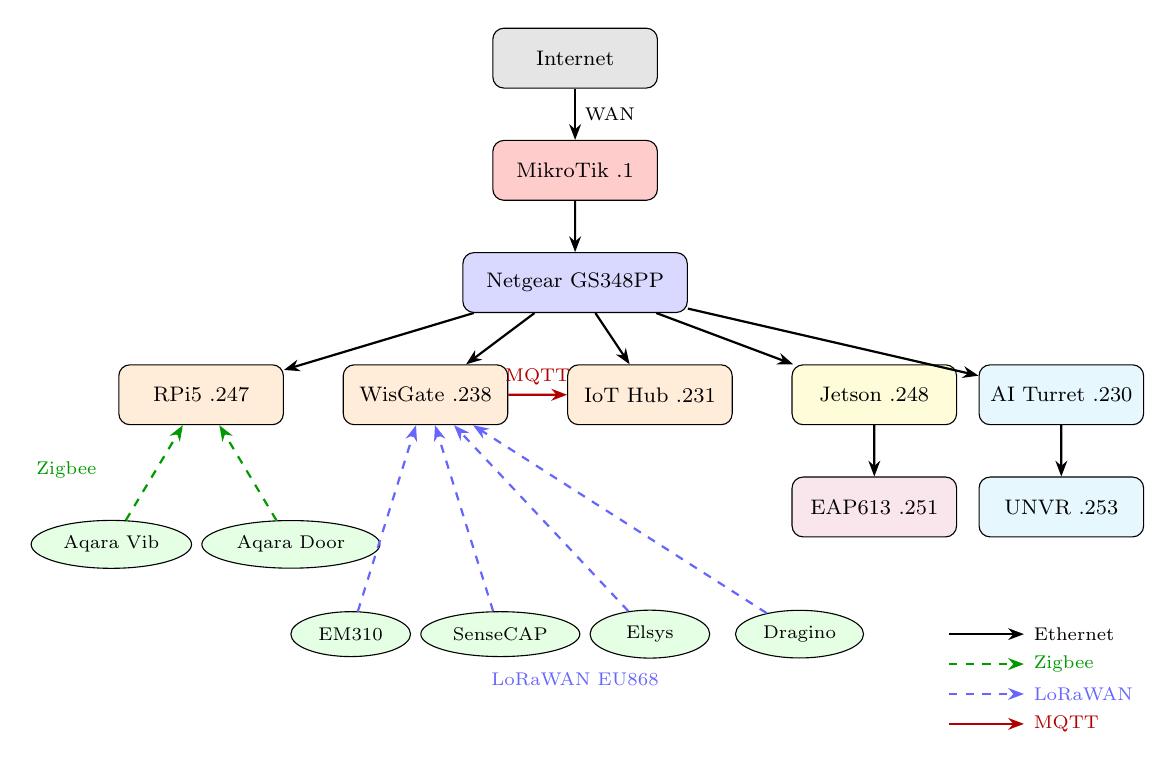
\begin{tikzpicture}[
    device/.style={rectangle, draw, rounded corners, minimum width=2.2cm, minimum height=0.8cm, font=\footnotesize},
    sensor/.style={ellipse, draw, minimum width=1.6cm, minimum height=0.6cm, font=\scriptsize, fill=green!10},
    link/.style={-{Stealth[length=2mm]}, thick},
    wireless/.style={-{Stealth[length=2mm]}, thick, dashed},
    scale=0.95, transform shape,
]

% Internet
\node[device, fill=gray!20] (internet) at (0, 7) {Internet};

% Core network
\node[device, fill=red!20] (mikrotik) at (0, 5.5) {MikroTik .1};
\node[device, fill=blue!15, minimum width=3cm] (netgear) at (0, 4) {Netgear GS348PP};

% Layer 2: Ethernet devices — left side (gateways)
\node[device, fill=orange!15] (rpi5) at (-5, 2.5) {RPi5 .247};
\node[device, fill=orange!15] (wisgate) at (-2, 2.5) {WisGate .238};
\node[device, fill=orange!15] (iothub) at (1, 2.5) {IoT Hub .231};

% Layer 2: Ethernet devices — right side (compute/infra)
\node[device, fill=yellow!15] (jetson) at (4, 2.5) {Jetson .248};
\node[device, fill=purple!10] (eap613) at (4, 1) {EAP613 .251};
\node[device, fill=cyan!10] (cam) at (6.5, 2.5) {AI Turret .230};
\node[device, fill=cyan!10] (nvr) at (6.5, 1) {UNVR .253};

% Layer 3: Zigbee sensors (under RPi5, spaced out)
\node[sensor] (aqara1) at (-6.2, 0.5) {Aqara Vib};
\node[sensor] (aqara2) at (-3.8, 0.5) {Aqara Door};

% Layer 3: LoRaWAN sensors (under WisGate/IoT Hub)
\node[sensor] (em310) at (-3, -0.7) {EM310};
\node[sensor] (sensecap) at (-1, -0.7) {SenseCAP};
\node[sensor] (elsys) at (1, -0.7) {Elsys};
\node[sensor] (dragino) at (3, -0.7) {Dragino};

% === Ethernet links ===
\draw[link] (internet) -- (mikrotik) node[midway, right, font=\scriptsize] {WAN};
\draw[link] (mikrotik) -- (netgear);
\draw[link] (netgear) -- (rpi5);
\draw[link] (netgear) -- (wisgate);
\draw[link] (netgear) -- (iothub);
\draw[link] (netgear) -- (jetson);
\draw[link] (netgear) -- (cam);
\draw[link] (jetson) -- (eap613);
\draw[link] (cam) -- (nvr);

% === Zigbee links (green dashed) ===
\draw[wireless, color=green!60!black] (aqara1) -- (rpi5);
\draw[wireless, color=green!60!black] (aqara2) -- (rpi5);
\node[font=\scriptsize, color=green!60!black] at (-6.8, 1.5) {Zigbee};

% === LoRaWAN links (blue dashed) ===
\draw[wireless, color=blue!60] (em310) -- (wisgate);
\draw[wireless, color=blue!60] (sensecap) -- (wisgate);
\draw[wireless, color=blue!60] (elsys) -- (wisgate);
\draw[wireless, color=blue!60] (dragino) -- (wisgate);
\node[font=\scriptsize, color=blue!60] at (0, -1.3) {LoRaWAN EU868};

% === MQTT link (red) ===
\draw[link, color=red!70!black] (wisgate) -- (iothub) node[midway, above, font=\scriptsize, color=red!70!black] {MQTT};

% === Legend ===
\draw[link, color=black] (5, -0.7) -- ++(1, 0) node[right, font=\scriptsize] {Ethernet};
\draw[wireless, color=green!60!black] (5, -1.1) -- ++(1, 0) node[right, font=\scriptsize] {Zigbee};
\draw[wireless, color=blue!60] (5, -1.5) -- ++(1, 0) node[right, font=\scriptsize] {LoRaWAN};
\draw[link, color=red!70!black] (5, -1.9) -- ++(1, 0) node[right, font=\scriptsize] {MQTT};

\end{tikzpicture}
\caption{NATO Smart City IoT Lab -- Physical network topology (192.xxx.x.0/24)}
\label{fig:topology}
\end{figure}

\subsection{Device Inventory}

\begin{table}[H]
\centering
\begin{tabular}{@{}llllp{4cm}@{}}
\toprule
\textbf{Device} & \textbf{Type} & \textbf{IP} & \textbf{OS/FW} & \textbf{Services} \\
\midrule
MikroTik RB5009 & Router & .1 & RouterOS 7.18.2 & FTP, SSH, Telnet, DNS, HTTP, WinBox \\
Netgear GS348PP & Switch & -- & -- & (no management interface) \\
RPi5 & Gateway & .247 & Debian 13 & SSH, MQTT (Mosquitto 2.0.21), Z2M UI \\
WisGate RAK7268 & Gateway & .238 & RAK FW & SSH (Dropbear 2020.81), HTTP/S (nginx 1.19.6) \\
IoT Hub (RPi5) & Gateway & .231 & Debian 13 & SSH, MQTT (Mosquitto 2.0.21) \\
Jetson Orin Nano & Compute & .248 & Ubuntu 22.04 & SSH \\
TP-Link EAP613 & AP & .251 & -- & HTTP/S, Management \\
\bottomrule
\end{tabular}
\caption{Attack surface devices with confirmed services}
\label{tab:devices}
\end{table}

% ================================================================
\section{System Architecture}
% ================================================================

The platform follows a layered data flow illustrated in Figure~\ref{fig:architecture}. YAML infrastructure definitions are parsed into Python dataclasses, populated into a directed graph backend, enriched with CVE data from the NIST NVD, analyzed for attack paths and risk scores, then consumed by a multi-phase LLM agent pipeline that produces pentest deliverables.

\begin{figure}[H]
\centering
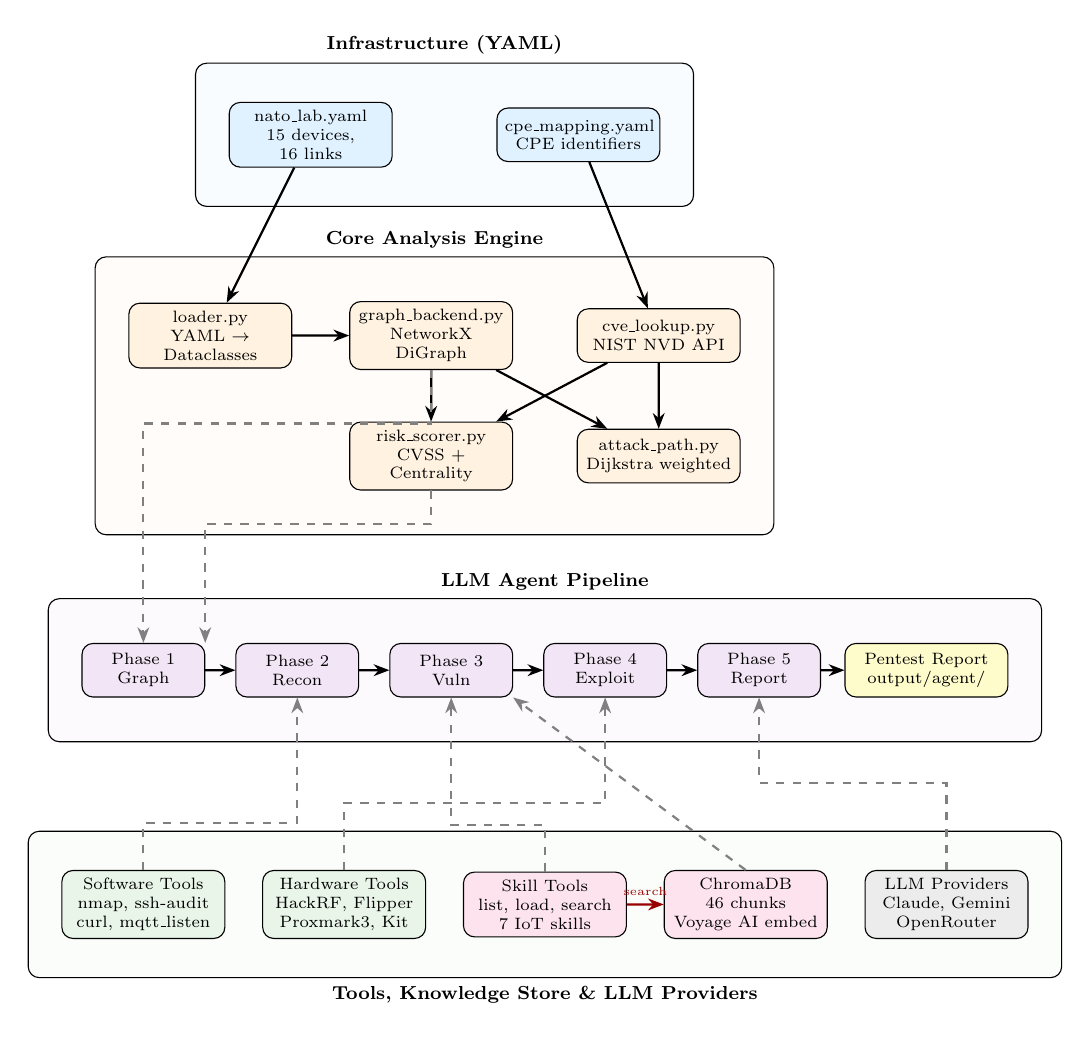
\begin{tikzpicture}[
    block/.style={rectangle, draw, rounded corners, minimum width=2.4cm, minimum height=0.8cm, font=\scriptsize, text width=2.2cm, align=center},
    phase/.style={rectangle, draw, rounded corners, minimum width=1.8cm, minimum height=0.8cm, font=\scriptsize, text width=1.6cm, align=center, fill=agentpurple},
    group/.style={rectangle, draw, rounded corners, inner sep=12pt},
    arrow/.style={-{Stealth[length=2mm]}, thick},
    darrow/.style={-{Stealth[length=2mm]}, thick, dashed, gray},
    scale=0.85, transform shape,
]

% === Layer 1: Infrastructure (y=0) ===
\node[block, fill=infrablue] (yaml) at (0, 0) {nato\_lab.yaml\\15 devices, 16 links};
\node[block, fill=infrablue] (cpe) at (4, 0) {cpe\_mapping.yaml\\CPE identifiers};

% === Layer 2: Core Engine (y=-3 to -5) ===
\node[block, fill=coreorange] (loader) at (-1.5, -3) {loader.py\\YAML $\rightarrow$ Dataclasses};
\node[block, fill=coreorange] (graph) at (1.8, -3) {graph\_backend.py\\NetworkX DiGraph};
\node[block, fill=coreorange] (cve) at (5.2, -3) {cve\_lookup.py\\NIST NVD API};
\node[block, fill=coreorange] (risk) at (1.8, -4.8) {risk\_scorer.py\\CVSS + Centrality};
\node[block, fill=coreorange] (attack) at (5.2, -4.8) {attack\_path.py\\Dijkstra weighted};

% === Layer 3: Agent Pipeline (y=-8) ===
\node[phase] (p1) at (-2.5, -8) {Phase 1\\Graph};
\node[phase] (p2) at (-0.2, -8) {Phase 2\\Recon};
\node[phase] (p3) at (2.1, -8) {Phase 3\\Vuln};
\node[phase] (p4) at (4.4, -8) {Phase 4\\Exploit};
\node[phase] (p5) at (6.7, -8) {Phase 5\\Report};

% === Output ===
\node[block, fill=yellow!20, minimum width=2cm] (report) at (9.2, -8) {Pentest Report\\output/agent/};

% === Layer 4: Tools & Knowledge (y=-11.5) ===
\node[block, fill=toolgreen] (sw) at (-2.5, -11.5) {Software Tools\\nmap, ssh-audit\\curl, mqtt\_listen};
\node[block, fill=toolgreen] (hw) at (0.5, -11.5) {Hardware Tools\\HackRF, Flipper\\Proxmark3, Kit};
\node[block, fill=knowledgepink] (skills) at (3.5, -11.5) {Skill Tools\\list, load, search\\7 IoT skills};
\node[block, fill=knowledgepink] (chroma) at (6.5, -11.5) {ChromaDB\\46 chunks\\Voyage AI embed};
\node[block, fill=gray!15] (llm) at (9.5, -11.5) {LLM Providers\\Claude, Gemini\\OpenRouter};

% === Arrows: Infrastructure -> Core ===
\draw[arrow] (yaml) -- (loader);
\draw[arrow] (cpe) -- (cve);
\draw[arrow] (loader) -- (graph);
\draw[arrow] (graph) -- (risk);
\draw[arrow] (graph) -- (attack);
\draw[arrow] (cve) -- (risk);
\draw[arrow] (cve) -- (attack);

% === Arrows: Core -> Pipeline ===
\draw[darrow] (graph.south) -- ++(0, -0.8) -| (p1.north);
\draw[darrow] (risk.south) -- ++(0, -0.5) -| (p1.north east);

% === Arrows: Pipeline flow ===
\draw[arrow, thick] (p1) -- (p2);
\draw[arrow, thick] (p2) -- (p3);
\draw[arrow, thick] (p3) -- (p4);
\draw[arrow, thick] (p4) -- (p5);
\draw[arrow] (p5) -- (report);

% === Arrows: Tools <-> Pipeline ===
\draw[darrow] (sw.north) -- ++(0, 0.7) -| (p2.south);
\draw[darrow] (hw.north) -- ++(0, 1.0) -| (p4.south);
\draw[darrow] (skills.north) -- ++(0, 0.7) -| (p3.south);
\draw[darrow] (chroma.north) -- (p3.south east);
\draw[darrow] (llm.north) -- ++(0, 1.3) -| (p5.south);

% === Skill -> ChromaDB link ===
\draw[arrow, color=red!60!black] (skills) -- (chroma) node[midway, above, font=\tiny, color=red!60!black] {search};

% === Group backgrounds with padding ===
\begin{scope}[on background layer]
    \node[group, fill=infrablue!20, inner ysep=14pt, fit=(yaml)(cpe), label={[font=\footnotesize\bfseries]above:Infrastructure (YAML)}] {};
    \node[group, fill=coreorange!20, inner ysep=16pt, fit=(loader)(graph)(cve)(risk)(attack), label={[font=\footnotesize\bfseries]above:Core Analysis Engine}] {};
    \node[group, fill=agentpurple!20, inner ysep=16pt, fit=(p1)(p2)(p3)(p4)(p5)(report), label={[font=\footnotesize\bfseries]above:LLM Agent Pipeline}] {};
    \node[group, fill=toolgreen!20, inner ysep=14pt, fit=(sw)(hw)(skills)(chroma)(llm), label={[font=\footnotesize\bfseries]below:Tools, Knowledge Store \& LLM Providers}] {};
\end{scope}

\end{tikzpicture}
\caption{Platform architecture -- data flow from YAML infrastructure to pentest report}
\label{fig:architecture}
\end{figure}

\subsection{Graph Backend}

The infrastructure is modeled as a NetworkX directed graph (\texttt{nx.DiGraph}). An abstract \texttt{GraphBackend} ABC defines the query interface (\texttt{get\_neighbors}, \texttt{find\_all\_paths}, \texttt{get\_attack\_surface}, \texttt{to\_dict}), allowing alternative backends (Neo4j, Memgraph) to be swapped in without changing analysis code. The attack surface is defined as devices exposing services (open ports). Sensors with only wireless protocols (LoRaWAN, Zigbee) and no IP services are excluded.

\subsection{CVE Enrichment and Risk Scoring}

A CPE mapping file (\texttt{infrastructure/cpe\_mapping.yaml}) maps devices and services to exact NVD identifiers. The CVE lookup module queries the NIST NVD API with rate limiting (5 sec/request) and parses CVSS 3.1/2.0 scores. Currently, 24 CVEs have been identified across 5 devices.

Risk scoring combines three factors: \textbf{CVSS maximum} (highest vulnerability score), \textbf{hop distance} (hops from Internet entry point), and \textbf{betweenness centrality} (how critical the device is as a network pivot). The highest-risk devices are MikroTik (6.6) and WisGate (5.6).

\subsection{Attack Path Analysis}

The attack path module implements Dijkstra-based weighted path analysis. Edge weights combine CVSS exploitability scores with protocol-specific factors:

\begin{table}[H]
\centering
\begin{tabular}{@{}lcl@{}}
\toprule
\textbf{Protocol} & \textbf{Factor} & \textbf{Rationale} \\
\midrule
Ethernet & 1.0 & Direct physical access, full bandwidth \\
WiFi & 0.9 & Wireless but standard IP stack \\
MQTT & 0.8 & Application layer, often unauthenticated \\
LoRaWAN & 0.6 & Encrypted (AES-128), limited bandwidth \\
Zigbee & 0.5 & Mesh network, key exchange vulnerability \\
\bottomrule
\end{tabular}
\caption{Protocol-specific edge weight factors}
\label{tab:protocols}
\end{table}

The scoring formula for a multi-hop attack path follows NIST's aggregation approach~\cite{nist_aggregation}:
\[
\text{Score}(\text{path}) = \prod_{i=1}^{n} P(\text{hop}_i) \times \text{impact}(\text{target}) \times \text{amplification}^{n-1}
\]

Where $P(\text{hop}_i)$ is the per-hop exploitation probability derived from CVSS exploitability, and the amplification factor captures the domino effect of chained vulnerabilities.

% ================================================================
\section{LLM Agent Pipeline}
% ================================================================

The core innovation of Q1 2026 is a multi-phase LLM agent pipeline inspired by the Shannon/LLMDFA approach~\cite{shannon_llmdfa} for automated security analysis. Unlike Q4 2025's single-query MCP approach, the pipeline decomposes the pentest workflow into 5 sequential phases, each with specialized tools and prompts.

\subsection{Pipeline Design}

\begin{table}[H]
\centering
\begin{tabular}{@{}clllc@{}}
\toprule
\textbf{Phase} & \textbf{Agent} & \textbf{Tools} & \textbf{Deliverable} & \textbf{Turns} \\
\midrule
1 & Graph Analysis & graph, deliverable & 01\_graph\_analysis.md & 3 \\
2 & Reconnaissance & graph, recon, deliverable & 02\_recon.md & 9 \\
3 & Vuln Analysis & graph, recon, deliverable & 03\_vuln\_*.json & 5--9 \\
4 & Exploitation & recon, deliverable & 04\_exploitation.md & -- \\
5 & Report & graph, deliverable & 05\_report.md & 4 \\
\bottomrule
\end{tabular}
\caption{Agent pipeline phases, tool assignments, and observed turn counts}
\label{tab:pipeline}
\end{table}

Each agent operates in an agentic loop: it receives a system prompt with context from previous phases, has access to its assigned tools, and iterates until it produces a deliverable. Phase 3 spawns per-device sub-agents (one for each attack surface device) to parallelize vulnerability analysis. The pipeline orchestrator manages phase sequencing, prerequisite validation, deliverable passing, and cost tracking.

\subsection{Tool System}

Tools are defined declaratively in YAML files. The tool loader parses definitions, generates JSON Schema for LLM tool calling, and auto-generates wrapper functions. Three tool types are supported:

\begin{itemize}
    \item \textbf{Subprocess tools} (5): auto-generated CLI wrappers (nmap, ssh-audit, curl, mosquitto\_sub, nvd\_lookup)
    \item \textbf{Hardware tools} (4): physical attack tools returning protocol-specific command suggestions
    \item \textbf{Graph/Skill/Deliverable tools} (12): Python functions for topology queries, knowledge search, and file I/O
\end{itemize}

\subsection{Hardware Attack Tools}

Four physical attack tools have been integrated as declarative YAML definitions. Unlike software tools that execute as subprocesses, hardware tools return protocol-specific commands and methodologies for the operator to execute manually.

\begin{table}[H]
\centering
\begin{tabular}{@{}llp{7cm}@{}}
\toprule
\textbf{Tool} & \textbf{Type} & \textbf{Capabilities} \\
\midrule
HackRF One & SDR (1--6 GHz) & Zigbee 802.15.4 sniffing (2.4 GHz), LoRaWAN EU868 capture, sub-GHz replay (433 MHz), GNU Radio integration \\
Flipper Zero & Multi-tool & Sub-GHz replay/bruteforce, RFID 125 kHz cloning, NFC 13.56 MHz emulation, IR replay, GPIO/UART bridging \\
Proxmark3 Easy & RFID/NFC & Mifare Classic cracking (darkside, hardnested, mfkey32), NTAG/DESFire read, EM4100/HID clone \\
Exploit IoT Kit & Hardware hacking & UART/JTAG/SWD debug, SPI/I2C flash dump, firmware extraction, voltage glitching \\
\bottomrule
\end{tabular}
\caption{Integrated hardware attack tools}
\label{tab:hardware}
\end{table}

\subsection{Knowledge Store and Skill Pipeline}

A ChromaDB-backed vector database provides semantic search over IoT security knowledge. The store uses Voyage AI embeddings (\texttt{voyage-3.5-lite}, 512 dimensions) with persistent storage. Two collections are maintained:

\begin{itemize}
    \item \textbf{skills}: 46 chunks from 7 IoT security skill files (MQTT, SSH, LoRaWAN, Zigbee, MikroTik, firmware, web), chunked by \texttt{\#\#} headings with context prefixes for RAG retrieval
    \item \textbf{cve\_knowledge}: populated at runtime via a cache-then-query pattern (search ChromaDB first, fetch from NVD on cache miss)
\end{itemize}

The skill pipeline works as follows. Each skill is a Markdown file with YAML frontmatter declaring metadata (name, tags, tools, device types) and structured sections (overview, methodology, commands, CVEs, verification steps). At ingestion time, skills are chunked by \texttt{\#\#} headings, prefixed with skill context (e.g., \texttt{[Skill: zigbee\_security] Zigbee/802.15.4 security assessment...}), and embedded into ChromaDB via Voyage AI. At query time, agents call \texttt{search\_knowledge("zigbee RF sniffing")} and receive the most relevant skill chunks ranked by cosine similarity. This RAG (Retrieval-Augmented Generation) approach means:

\begin{enumerate}
    \item Agents do not need the full skill text in their prompt (context window savings)
    \item Queries are fuzzy --- ``UART firmware dump'' returns firmware\_analysis chunks even without exact keyword matches
    \item New skills are automatically searchable after a single ingestion call
    \item Hardware tool references in skills (e.g., \texttt{tools: [hackrf\_capture]}) are preserved in chunk metadata, enabling tool-aware retrieval
\end{enumerate}

\subsection{Multi-Provider LLM Support}

The provider abstraction layer translates tool schemas between Anthropic (native \texttt{tool\_use}) and OpenAI-compatible APIs (function calling). Supported providers include Anthropic (Claude), OpenRouter (Gemini, Mistral), MiniMax, GLM, and Qwen. Per-model pricing tables enable cost tracking across providers.

% ================================================================
\section{Initial Results}
% ================================================================

The pipeline was executed on the physical lab on March 16, 2026, using Google Gemini 3 Flash Preview via OpenRouter. The full run completed in 23 minutes across 50 tool-calling turns at a total cost of \$0.38.

\subsection{Execution Metrics}

\begin{table}[H]
\centering
\begin{tabular}{@{}lccccc@{}}
\toprule
\textbf{Phase} & \textbf{Turns} & \textbf{Tool Calls} & \textbf{Input Tokens} & \textbf{Cost} & \textbf{Duration} \\
\midrule
Graph Analysis & 3 & 7 & 12K & \$0.01 & 16s \\
Reconnaissance & 9 & 18 & 335K & \$0.17 & 11m 23s \\
Vuln Analysis (6 devices) & 34 & 68 & 308K & \$0.18 & 11m 10s \\
Report & 4 & 6 & 19K & \$0.02 & 18s \\
\midrule
\textbf{Total} & \textbf{50} & \textbf{99} & \textbf{674K} & \textbf{\$0.38} & \textbf{23m 20s} \\
\bottomrule
\end{tabular}
\caption{Pipeline execution metrics (Gemini 3 Flash Preview, March 16, 2026)}
\label{tab:execution}
\end{table}

\subsection{Key Findings}

The agent autonomously discovered and documented the following vulnerabilities:

\begin{table}[H]
\centering
\begin{tabular}{@{}llllc@{}}
\toprule
\textbf{ID} & \textbf{Device} & \textbf{Type} & \textbf{Service} & \textbf{Severity} \\
\midrule
MISCONF-01 & rpi5 & Auth Bypass & MQTT (1883) & CRITICAL \\
CVE-2023-51767 & rpi5 / iot\_hub & DoS / Injection & Mosquitto & HIGH \\
CVE-2021-23017 & wisgate & RCE & nginx 1.19.6 & HIGH \\
CVE-2021-3014 & mikrotik & DNS Cache Poison & RouterOS & MEDIUM \\
CVE-2019-9511 & jetson & Resource Exhaustion & HTTP/2 & MEDIUM \\
\bottomrule
\end{tabular}
\caption{Vulnerabilities discovered by the agent pipeline}
\label{tab:vulns}
\end{table}

\textbf{Critical finding}: The MQTT broker on RPi5 (192.xxx.x.247:1883) accepts \textbf{anonymous connections}. The agent confirmed this by running \texttt{mqtt\_listen} and successfully receiving live Zigbee sensor data (Aqara vibration and door sensors) without any credentials. This allows any device on the LAN to intercept all smart city sensor data and potentially inject commands.

\subsection{Attack Paths Identified}

The agent identified two primary multi-hop attack paths:

\begin{enumerate}
    \item \textbf{Data Exfiltration}: Internet $\rightarrow$ MikroTik (CVE-2021-3014) $\rightarrow$ Netgear $\rightarrow$ RPi5 (anonymous MQTT) -- allows interception of all sensor data
    \item \textbf{Infrastructure Takeover}: Internet $\rightarrow$ MikroTik $\rightarrow$ Netgear $\rightarrow$ WisGate (CVE-2021-23017) -- nginx RCE could disrupt LoRaWAN communications
\end{enumerate}

\subsection{Risk Scores}

\begin{table}[H]
\centering
\begin{tabular}{@{}lcccc@{}}
\toprule
\textbf{Device} & \textbf{Risk Score} & \textbf{Max CVSS} & \textbf{Centrality} & \textbf{Hops from Internet} \\
\midrule
mikrotik & 6.6 & 7.5 & 0.13 & 1 \\
wisgate & 5.6 & 7.7 & 0.47 & 3 \\
rpi5 & 5.3 & 9.3 & 0.25 & 3 \\
iot\_hub & 4.1 & 9.3 & 0.00 & 3 \\
netgear & 3.0 & 0.0 & 0.72 & 2 \\
\bottomrule
\end{tabular}
\caption{Device risk scores combining CVSS, centrality, and hop distance}
\label{tab:risk}
\end{table}

\subsection{Model vs Reality Discrepancies}

The reconnaissance phase revealed discrepancies between the YAML model and actual network state, demonstrating the value of active scanning:

\begin{itemize}
    \item SSH versions updated on RPi5 and IoT Hub (10.0p1 $\rightarrow$ 10.0p2)
    \item WisGate port 80 is a redirect to HTTPS (443), not a standalone HTTP service
    \item MikroTik and EAP613 are unreachable to nmap scans (firewall filtering)
    \item Two active Zigbee sensors discovered via Z2M API (Aqara vibration + door)
\end{itemize}

\subsection{Remediation Priorities}

The agent generated prioritized recommendations:

\begin{enumerate}
    \item \textbf{IMMEDIATE}: Disable anonymous MQTT access on RPi5 and IoT Hub (configure Mosquitto authentication)
    \item \textbf{IMMEDIATE}: Update WisGate firmware (nginx 1.19.6 and Dropbear 2020.81 have known CVEs)
    \item \textbf{SHORT TERM}: Disable unused MikroTik services (Telnet, FTP); restrict WinBox to management VLAN
    \item \textbf{SHORT TERM}: Upgrade OpenSSH on Jetson (8.9p1 $\rightarrow$ current)
    \item \textbf{IMPROVEMENT}: Network segmentation -- IoT gateways in dedicated VLAN
\end{enumerate}

% ================================================================
\section{Comparative Analysis}
% ================================================================

\subsection{Comparison with Traditional Vulnerability Scanners}

\begin{table}[H]
\centering
\begin{tabular}{@{}lp{3.5cm}p{3.5cm}p{3.5cm}@{}}
\toprule
\textbf{Capability} & \textbf{Traditional Scanners} (Nessus, Qualys) & \textbf{Q4 2025} (Neo4j + MCP) & \textbf{Q1 2026} (Agent Pipeline) \\
\midrule
Vulnerability detection & Per-device CVE scan & CPE-based NVD lookup & CPE lookup + active recon validation \\
Attack path analysis & None (device-centric) & Basic graph traversal & Dijkstra-weighted multi-hop chains \\
IoT protocol support & Limited (mostly IP) & Protocol metadata only & LoRaWAN, Zigbee, MQTT active testing \\
RF/Hardware attacks & None & None & HackRF, Flipper, Proxmark3 guidance \\
AI integration & None & Single MCP query & 5-phase agentic pipeline \\
Report generation & Template-based & Manual & Fully automated per-run \\
Cost per assessment & \$5K+ license/year & Free (self-hosted) & \$0.38 per run (API tokens) \\
\bottomrule
\end{tabular}
\caption{Platform comparison with existing approaches}
\label{tab:comparison}
\end{table}

\subsection{Comparison with IoT Pentest Frameworks}

The platform's hybrid approach combines elements from several established methodologies:

\begin{itemize}
    \item \textbf{OWASP ISTG}: Component-based device model (wireless interfaces, internal interfaces, firmware) -- adopted in skill organization
    \item \textbf{PTES}: Phase-based workflow (reconnaissance $\rightarrow$ exploitation $\rightarrow$ reporting) -- directly maps to the 5-phase pipeline
    \item \textbf{AttifyOS/Kali}: Domain-based tool organization -- adopted for hardware tool YAML definitions
    \item \textbf{Shannon/LLMDFA}: Multi-agent LLM analysis with tool calling -- core inspiration for the pipeline architecture
\end{itemize}

The key differentiator is the \textbf{graph-based attack path analysis}: while traditional scanners identify vulnerabilities in isolation, the platform discovers how an attacker could chain a DNS cache poisoning on MikroTik (MEDIUM severity) with an anonymous MQTT broker (CRITICAL) and a LoRaWAN gateway RCE (HIGH) to compromise the entire smart city sensor network through a 3-hop lateral movement chain.

% ================================================================
\section{Testing and Validation}
% ================================================================

The platform maintains 193 automated tests across 14 test files, covering all modules from YAML loading to hardware tool integration.

\begin{table}[H]
\centering
\begin{tabular}{@{}lcp{6cm}@{}}
\toprule
\textbf{Test File} & \textbf{Tests} & \textbf{Coverage} \\
\midrule
test\_loader.py & 14 & YAML loading, graph construction, paths \\
test\_attack\_path.py & 16 & Edge weights, Dijkstra paths, pivots \\
test\_risk\_scorer.py & 11 & CVSS, centrality, hop distance \\
test\_tool\_loader.py & 17 & YAML parsing, schema gen, hardware tools \\
test\_agent\_tools.py & 24 & Recon tools, graph tools, provider \\
test\_pipeline.py & 14 & Tool resolution, dry-run, prerequisites \\
test\_skill\_tools.py & 9 & Skill listing, loading, frontmatter \\
Other (7 files) & 88 & CVE lookup, cost tracker, validators, etc. \\
\bottomrule
\end{tabular}
\caption{Test suite summary (193 tests, all passing)}
\label{tab:tests}
\end{table}

% ================================================================
\section{Next Steps (Q2 2026)}
% ================================================================

\begin{itemize}
    \item \textbf{Progressive pentesting}: execute exploitation phase on the real lab -- safe tests first (MQTT anonymous access, SSH default creds, Terrapin scan), then destructive tests on Docker containers reproducing vulnerable services (nginx:1.19.6, Dropbear 2020.81, MikroTik CHR)
    \item \textbf{NFC access control}: integrate a PN532 NFC reader on RPi for physical access control simulation; test badge cloning with Proxmark3
    \item \textbf{RF testing}: HackRF-based Zigbee 802.15.4 sniffing on channels 11--26 and LoRaWAN EU868 capture using GNU Radio pipelines (\texttt{gr-ieee802-15-4}, \texttt{gr-lora})
    \item \textbf{Firmware extraction}: UART/JTAG testing on WisGate gateway using the Exploit IoT Kit
    \item \textbf{Multi-hop attack validation}: end-to-end exploitation chains combining network, RF, and physical access vectors
    \item \textbf{Agent pipeline refinement}: add exploitation phase (Phase 4) with safe test execution; improve per-device vulnerability analysis accuracy
\end{itemize}

% ================================================================
\section{Conclusion}
% ================================================================

Q1 2026 has transformed the platform from a graph-database prototype into a fully operational IoT pentest automation system. The key achievements are:

\begin{enumerate}
    \item \textbf{Real lab deployment}: 15 physical devices modeled and actively scanned (vs. simulated JSON in Q4 2025)
    \item \textbf{Automated pentest pipeline}: 5-phase LLM agent produces complete pentest reports for \$0.38 in 23 minutes
    \item \textbf{Actionable findings}: anonymous MQTT access confirmed, multi-hop attack chains identified, prioritized remediation generated
    \item \textbf{Hardware tool integration}: 4 physical attack tools (HackRF, Flipper Zero, Proxmark3, Exploit IoT Kit) ready for RF and hardware testing in Q2
    \item \textbf{Knowledge-augmented agents}: ChromaDB semantic search over 7 IoT security skills enables context-aware vulnerability analysis
\end{enumerate}

The platform demonstrates that LLM-powered agentic pipelines can automate a significant portion of the IoT pentest workflow, from topology analysis to report generation, while maintaining the flexibility to incorporate physical attack vectors through hardware tool integration.

% ================================================================
\begin{thebibliography}{9}

\bibitem{nist_aggregation}
NIST, \emph{Aggregating Vulnerability Metrics in Enterprise Networks using Attack Graphs}, 2014.
\url{https://tsapps.nist.gov/publication/get_pdf.cfm?pub_id=926022}

\bibitem{shannon_llmdfa}
X. Li et al., \emph{LLM-Assisted Static Analysis for Detecting Security Vulnerabilities}, arXiv:2405.17238, 2024.

\bibitem{first_cvss}
FIRST, \emph{CVSS v3.1 Specification Document}.
\url{https://www.first.org/cvss/v3-1/specification-document}

\bibitem{owasp_istg}
OWASP, \emph{IoT Security Testing Guide}.
\url{https://owasp.org/owasp-istg/}

\bibitem{picus}
Picus Security, \emph{Attack Path Analysis Explained}.
\url{https://www.picussecurity.com/resource/blog/what-is-attack-path-analysis}

\bibitem{domino}
Software Secured, \emph{The Domino Effect: Chaining Medium and Low Vulnerabilities}.
\url{https://www.softwaresecured.com/post/the-domino-effect-chaining-medium-and-low-vulnerabilities-is-the-path-to-critical-breaches}

\end{thebibliography}

\end{document}